% Preamble
\documentclass[specialist,
    substylefile = spbu_report.rtx,
    subf,href,colorlinks=true, 12pt]{disser}

% Packages
\usepackage[a4paper, includefoot,
    left=3cm, right=1.5cm,
    top=2cm, bottom=2cm,
    headsep=1cm, footskip=1cm]{geometry}
\usepackage{amsmath}
\usepackage{amssymb}
\usepackage[T2A]{fontenc}
\usepackage[utf8]{inputenc}
\usepackage[english, russian]{babel}
\usepackage{pdfpages}
\usepackage{graphicx}
\usepackage{wrapfig}
\usepackage{amsthm}
\usepackage{framed}
\usepackage{xcolor}
\usepackage{color}
\usepackage{fancyvrb}
%\usepackage{nath}
%\usepackage{cnbwp}
%\usepackage{hyperref}

\setcounter{tocdepth}{2}
\graphicspath{{./img}}

\theoremstyle{plain}
\newtheorem{statement}{Утверждение}[section]
\newtheorem{corollary}{Следствие}[statement]

\theoremstyle{definition}
\newtheorem{definition}{Определение}[section]
\newtheorem{property}{Свойство}[section]

\theoremstyle{remark}
\newtheorem*{remark}{Замечание}

% Document
\begin{document}

    \title{Учебная практика 3 (научно-исследовательская работа)}
    \topic{<<Tensor SSA для анализа временного ряда>>}
    \author{Хромов Никита Андреевич}
    \date{\number\year}
    \institution{
        Санкт-Петербургский государственный университет\\
        Прикладная математика и информатика
    }
    \group{20.Б04-мм}
    \sa       {Голяндина~Н.\,Э.}
    \sastatus {к.\,ф.-м.\,н., доцент}
    \city{Санкт-Петербург}
    \maketitle

    \tableofcontents


    \section{Введение}\label{sec:intro}
    Здесь должно быть введение.
    \newpage


    \section{Описание метода TSSA}\label{sec:tssa-method-description}
    Дан временной ряд $F$ длины $N$
    \[F=(f_1,f_2,\ldots,f_N).\]
    На первом этапе выбираются два натуральных параметра $I, L: I+L-1\leqslant N$, по ним высчитывается третий параметр $J=N-I-L+2$.
    С учётом этих параметров строится траекторный тензор $\mathcal X$ размерности $I\times L \times J$ следующим образом
    \[\mathcal{X}_{i,l,j}=f_{i+l+j-2}\qquad i\in \overline{1:I},\, l \in\overline{1:L},\, j \in\overline{1:J}.\]
    Слои тензора будут иметь следующий вид
    \[\mathcal{X}_{,,j}=
    \begin{pmatrix}
        f_j       & f_{j+1} & \ldots & f_{j+L-1}   \\
        f_{j+1}   & \ddots  &        & \vdots      \\
        \vdots    &         & \ddots & \vdots      \\
        f_{j+I-1} & \ldots  & \ldots & f_{j+I+L-2}
    \end{pmatrix},\]
    \[\mathcal{X}_{,l,}=
    \begin{pmatrix}
        f_l       & f_{l+1} & \ldots & f_{l+J-1}   \\
        f_{l+1}   & \ddots  &        & \vdots      \\
        \vdots    &         & \ddots & \vdots      \\
        f_{l+I-1} & \ldots  & \ldots & f_{l+I+J-2}
    \end{pmatrix},\]
    \[\mathcal{X}_{i,,}=
    \begin{pmatrix}
        f_i       & f_{i+1} & \ldots & f_{i+J-1}   \\
        f_{i+1}   & \ddots  &        & \vdots      \\
        \vdots    &         & \ddots & \vdots      \\
        f_{i+L-1} & \ldots  & \ldots & f_{i+L+J-2}
    \end{pmatrix}.\]

    На втором этапе к полученному тензору применяется HOSVD~\cite{hosvd} "--- тензорное разложение,
    являющееся обобщением SVD на большие размерности.
    Результатом разложения является набор из одного тензора $\mathcal{Z}$ размерности $I\times L\times J$ и трёх
    ортогональных матриц $\mathbf{U}^{(1)},\, \mathbf{U}^{(2)},\, \mathbf{U}^{(3)}$ размерностей
    $I\times I,\, L\times L,\, J\times J$ соответственно.

    Этот набор удовлетворяет равенству
    \begin{equation}
        \mathcal{X}=\mathcal{Z}\times_1 \mathbf{U}^{(1)}\times_2 \mathbf{U}^{(2)} \times_3 \mathbf{U}^{(3)},\label{eq:trajectory-hosvd}
    \end{equation}
    где $\times_n$ "--- произведение тензора на матрицу по $n$-му измерению.
    Оно определяется следующим образом: пусть $\mathcal A$ "--- тензор размерности
    $I_1\times I_2\times\ldots\times I_K$, $\mathbf U$ "--- матрица размерности $J_n\times I_n$, тогда
    $\mathcal{A}\times_n \mathbf U$ "--- тензор размерности $I_1\times I_2\times\ldots\times I_{n-1}
    \times J_n\times I_{n+1}\times \ldots\times I_K$, который считается по формуле
    \[(\mathcal{A}\times_n \mathbf U)_{i_1 i_2\ldots i_{n-1}j_n i_{n+1}\ldots i_K} = \sum_{i_n=1}^{I_n} a_{i_1 i_2\ldots
    i_{n-1}i_n i_{n+1} \ldots i_K} u_{j_n i_n}.\]

    Обозначим за $\mathcal Z_{i_n=\alpha}$ подтензор тензора $\mathcal Z$, полученный фиксированием индекса $i_n=\alpha$.
    Тензор $\mathcal Z$ удовлетворяет следующим свойствам:
    \begin{enumerate}
        \item подтензоры $\mathcal Z_{i_n=\alpha}$ и $\mathcal Z_{i_n=\beta}$ ортогональны для всех возможных значений
        $n,\, \alpha,\, \beta: \alpha\ne\beta$:
        \[\langle\mathcal Z_{i_n=\alpha},\mathcal Z_{i_n=\beta}\rangle=0 \qquad \alpha\ne\beta,\]
        \item подтензоры расположены в порядке убывания их нормы Фробениуса:
        \[\|\mathcal Z_{i_n=1}\|\geqslant\|\mathcal Z_{i_n=2}\| \geqslant \ldots \geqslant\|\mathcal Z_{i_n=I_n}\|\]
        для всех $n\in \{1,\, 2,\, 3\}$, где $I_1=I,\, I_2=L,\, I_3=J$.
    \end{enumerate}
    \begin{definition}
        \label{def:singular-value}
        Обозначим $\sigma_i^{(n)}=\|\mathcal Z_{i_n=i}\|$ и будем называть $\sigma_i^{(n)}$ $i$-м сингулярным числом
        тензора $\mathcal X$ по измерению $n$.
    \end{definition}
    \begin{definition}
        \label{def:singular-tensor}
        Векторы $\mathbf U_i^{(n)}$ будем называть $i$-м сингулярным вектором тензора $\mathcal X$ по измерению $n$.
    \end{definition}

    Разложение~\eqref{eq:trajectory-hosvd} можно представить в виде суммы
    \[
        \mathcal{X}=\sum_{i=1}^{I} \sum_{l=1}^{L} \sum_{j=1}^{J} \mathcal{Z}_{i,l,j} \mathbf{U}^{(1)}_{i}
        \circ \mathbf{U}^{(2)}_{l} \circ \mathbf{U}^{(3)}_{j}.
    \]
    Такой вид позволяет провести третий этап "--- группировку.
    Множество индексов $\mathfrak{S}=\{1,\, 2\,\ldots,\, \min(I, L, J)\}$ разбивается по смыслу на непересекающиеся множества
    \[\mathfrak{S}=\bigcup_{k=1}^{m}\mathfrak{S}_k \qquad \mathfrak{S}_k\cap \mathfrak{S}_l =\emptyset,\, k\ne l.\]
    По каждой из групп строятся тензоры
    \begin{equation}
        \mathcal{X}^{(\mathfrak{S}_k)}=\sum_{i \in \mathfrak{S}_k} \sum_{l\in \mathfrak{S}_k} \sum_{j\in \mathfrak{S}_k}
        \mathcal{Z}_{i,l,j} \mathbf{U}^{(1)}_{i}\circ \mathbf{U}^{(2)}_{l} \circ \mathbf{U}^{(3)}_{j}.\label{eq:tens-group}
    \end{equation}

    На четвёртом этапе, по каждому тензору вида~\eqref{eq:tens-group}, полученному после этапа группировки, восстанавливается ряд.
    По соображениям построения траекторного тензора, компоненты ряда восстанавливаются усреднением вдоль плоскостей $i+l+j=\operatorname{const}$.
    Другими словами, компоненты восстановленного ряда $F^{(k)}=F^{(\mathfrak{S}_k)}$ высчитываются по формуле
    \[
        f^{(k)}_n=\frac{1}{\#\mathfrak{M}_n}\sum_{(i,l,j)\in \mathfrak{M}_n} \mathcal{X}^{(\mathfrak{S}_k)}_{i,l,j},\qquad n\in \overline{1:N},
    \]
    где $\mathfrak{M}_n=\{(i,\, l,\, j) | 1\leqslant i \leqslant I,\, 1\leqslant l \leqslant L,\, 1\leqslant j \leqslant J,\, i+l+j-2=n\}$.

    Результатом метода является набор временных рядов $F^{(1)},\ldots,\, F^{(m)}$ такой, что ${F=\sum_{k=1}^{m}F^{(k)}}$.


    \section{Свойства HOSVD}\label{sec:hosvd-properties}
    Многие свойства метода SSA являются следствиями свойств SVD\@.
    В свою очередь, многие свойства HOSVD являются аналогами свойств SVD\@.
    Таким образом, аналогичность свойств SSA и TSSA может быть выведена из аналогичности некоторых свойств SVD и HOSVD\@.
    \begin{statement}
        Вычисление \emph{HOSVD} тензора $\mathcal{A}$ с $N$ размерностями сводится к вычислению \emph{SVD} на $N$ матрицах $\mathbf{A}_{(n)}$,
        которые вычисляются развёрткой тензора по $n$-му измерению.
    \end{statement}
    Другими словами, если $\mathcal{A}$ "--- тензор размерности $I_1\times I_2\times\ldots\times I_N$, то его развёртка
    по $n$-му измерению "--- это матрица $\mathbf{A}_{(n)}$ размерности $I_n\times I_{n+1}I_{n+2}\ldots I_{N}I_{1}I_{2}\ldots
    I_{n-1}$, в которой элемент $a_{i_1 i_2\ldots i_N}$ тензора содержится в строке $i_n$ и столбце с номером равным
    \[\begin{aligned}
          &(i_{n+1} - 1)I_{n+2}I_{n+3}\ldots I_{N}I_1 I_2\ldots I_{n-1} + (i_{n+2} - 1)I_{n+3}I_{n+4}\ldots I_N I_1 I_2 \ldots
          I_{n-1} + \dots \\
          &+(i_N - 1)I_1 I_2 \ldots I_{n-1} + (i_1 - 1)I_2 I_3\ldots I_{n-1} + (i_2 - 1)I_3 I_4\ldots I_{n-1} + \dots + i_{n-1}.
    \end{aligned}
    \]

    \begin{figure}[!h]
        \centering
        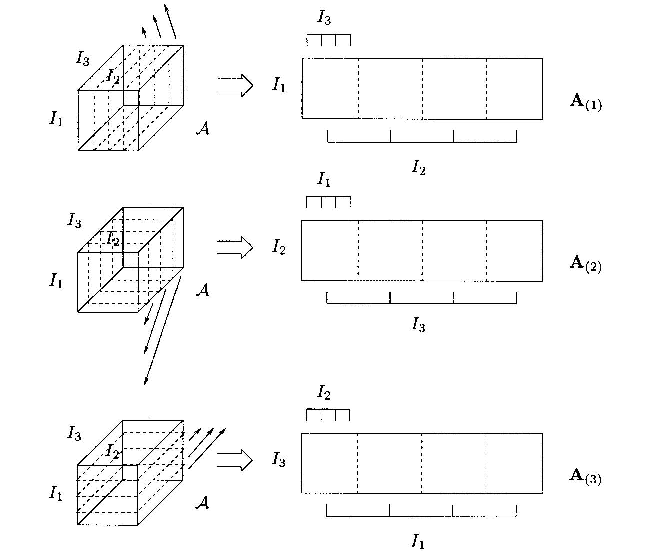
\includegraphics[width=\textwidth]{unfolding}
        \caption{Развёртка тензора $\mathcal{A}$ размерности $I_1\times I_2 \times I_3$ в матрицы $\mathbf{A}_{(1)},\,
        \mathbf{A}_{(2)},\, \mathbf{A}_{(3)}$ размерностей $I_1\times (I_2 I_3),\, I_2\times (I_3 I_1),\, I_3\times (I_1 I_2)$
            соответственно}
        \label{fig:unfolding}
    \end{figure}

    К каждой из полученных матриц применяется SVD, в результате чего получаются $N$ матриц $\mathbf{U}^{(n)}$,
    составленных из левых сингулярных векторов соответствующих развёрток.
    Затем находится тензор сингулярных чисел
    \[\mathcal{Z}=\mathcal{A}\times_1 \mathbf{U}^{(1)^\mathrm{H}}\times_2 \mathbf{U}^{(2)^\mathrm{H}}\ldots \times_N
    \mathbf{U}^{(N)^\mathrm{H}}.\]
    В результате получается искомое разложение
    \[\mathcal{A} = \mathcal{Z}\times_1 \mathbf{U}^{(1)}\times_2 \mathbf{U}^{(2)}\ldots \times_N \mathbf{U}^{(N)}.\]

    Из-за этой связи HOSVD с обычным матричным SVD для многих свойств SVD существуют аналогичные свойства HOSVD\@.
    \begin{property}[Единственность]
        \leavevmode
        \begin{enumerate}
            \item Все сингулярные числа по каждому измерению определяются однозначно.
            \item Если сингулярные числа по измерению $n$ различны, то сингулярные векторы по измерению $n$ определены
            в точности до умножения на коэффициент единичной нормы.
            Если $U_\alpha^{(n)}$ умножается на $e^{j\theta}$, то $\mathcal{Z}_{i_n=\alpha}$ должен быть умножен на обратный
            коэффициент $e^{-j\theta}$.
        \end{enumerate}
        Сингулярные векторы по измерению $n$, соответствующие одному и тому же сингулярному числу по измерению $n$,
        могут быть заменены любой унитарной линейной комбинацией.
        Соответствующие подтензоры $\{\mathcal{Z}_{i_n=\alpha}\}$ должны быть пересчитаны обратным образом.
        Формально $\mathbf{U}^{(n)}$ можно заменить на $\mathbf{U}^{(n)}\mathbf{Q}$, где $\mathbf{Q}$ "--- блочно-диагональная
        матрица, состоящая из унитарных блоков, в которой блочное разбиение соответствует разбиению $\mathbf{U}^{(n)}$
        на наборы сингулярных векторов по измерению $n$ соответствующих одинаковым сингулярным значениям по измерению $n$.
        При этом тензор $\mathcal{Z}$ должен быть заменён на $\mathcal{Z}\times_{n} \mathbf{Q}^{\mathrm{H}}$.

        В случае вещественно-значных тензоров единственность имеется в точности до знака, что соответствует
        умножению на унитарную матрицу.
    \end{property}

    \begin{property}[Обобщение]
        HOSVD тензора второго порядка сводится к его матричному SVD\@.
    \end{property}

    Перед формулировкой следующих свойств необходимо ввести определение.
    \begin{definition}[$n$-ранг]
        $n$-рангом тензора $\mathcal{A}$ называется размерность векторного пространства, порождённого векторами измерения $n$ этого тензора.
        Обозначается $R_n=\operatorname{rank}_{n}(\mathcal{A})$.
    \end{definition}

    \begin{remark}
        В отличие от матричного случая, $n$-ранги тензора порядка выше $2$ могут в общем случае отличаться.
    \end{remark}

    \begin{property}[Связь $n$-ранга тензора и ранга его развёртки по измерению $n$]
        Векторы размерности $n$ тензора $\mathcal{A}$ являются столбцами его развёртки по измерению $n$ и выполняется равенство
        \[\operatorname{rank}_{n}(\mathcal{A})=\operatorname{rank}(\mathbf{A}_{(n)}).\]
    \end{property}

    \begin{property}[Связь $n$-ранга тензора и его HOSVD]
        Пусть имеется HOSVD тензора $\mathcal{A}$ размерности $I_1\times I_2\times \ldots \times I_N$
        \[\mathcal{A} = \mathcal{Z}\times_1 \mathbf{U}^{(1)}\times_2\mathbf{U}^{(2)}\times_3\ldots \times_{N}\mathbf{U}^{(N)},\]
        тогда, по определению, тензор $\mathcal{Z}$ удовлетворяет свойству упорядоченности сингулярных чисел
        \[\|\mathcal{Z}_{i_n=1}\|\geqslant\|\mathcal{Z}_{i_n=2}\|\geqslant\ldots \geqslant \|\mathcal{Z}_{i_n=I_n}\|\]
        для всех $n\in \overline{1:N}$.
        Обозначим $r_n$ "--- наибольший индекс такой, что $\|\mathcal{Z}_{i_n=r_n}\|>0$.
        Тогда
        \begin{equation}
            \operatorname{rank}_n(\mathcal{A})=r_n.\label{eq:n-rank}
        \end{equation}
    \end{property}

    Все утверждения выше и их доказательства приведены в статье~\cite{hosvd}.

    \section{Свойства TSSA}\label{sec:tssa-properties}
    В силу аналогичности свойств SVD и HOSVD, многие определения и свойства из теории SSA можно перенести на тензорный случай.
    \begin{statement}
        \label{state:separability}
        $\tilde{F}=(\tilde{f}_1,\ldots , \tilde{f}_N)$, $\hat{F}=(\hat{f}_1,\ldots , \hat{f}_N)$ "--- временные ряды длины $N$.
        Пусть ряд $F$ является суммой этих рядов.
        Траекторные тензоры рядов равны соответственно: $\tilde{\mathcal{X}},\, \hat{\mathcal{X}},\, \mathcal{X}$.
        Тогда существует сингулярное разложение тензора $\mathcal{X}$ с параметрами $I, L$, которое можно представить
        в виде суммы сингулярных разложений тензоров $\tilde{\mathcal{X}}$ и $\hat{\mathcal{X}}$ с теми же параметрами
        в том и только том случае, когда взаимно ортогональны все подряды рядов $\tilde{F}$ и $\hat{F}$
        длины $I,\, L,\, J=N-I-L+2$, то есть
        \begin{enumerate}
            \item $\tilde{f}_{k}\hat{f}_m + \ldots + \tilde{f}_{k+I-1} \hat{f}_{m+I-1}=0 \qquad \forall k,\, m\in\overline{1:N-I+1}$,
            \item $\tilde{f}_{k}\hat{f}_m + \ldots + \tilde{f}_{k+L-1} \hat{f}_{m+L-1}=0 \qquad \forall k,\, m\in\overline{1:N-L+1}$,
            \item $\tilde{f}_{k}\hat{f}_m + \ldots + \tilde{f}_{k+J-1} \hat{f}_{m+J-1}=0 \qquad \forall k,\, m\in\overline{1:N-J+1}$.
        \end{enumerate}
    \end{statement}
    \begin{proof}
        Сингулярные разложения тензоров $\mathcal{X}, \tilde{\mathcal{X}}, \hat{\mathcal{X}}$ могут быть представлены в виде
        следующих сумм:
        \[
            \begin{aligned}
                \mathcal{X}=\sum_{i=1}^{I} \sum_{l=1}^{L} \sum_{j=1}^{J} \mathcal{Z}_{i,l,j} \mathbf{U}^{(1)}_{i}
                \circ \mathbf{U}^{(2)}_{l} \circ \mathbf{U}^{(3)}_{j},\\
                \tilde{\mathcal{X}}=\sum_{i=1}^{I} \sum_{l=1}^{L} \sum_{j=1}^{J} \tilde{\mathcal{Z}}_{i,l,j}
                \tilde{\mathbf{U}}^{(1)}_{i} \circ \tilde{\mathbf{U}}^{(2)}_{l} \circ \tilde{\mathbf{U}}^{(3)}_{j},\\
                \hat{\mathcal{X}}=\sum_{i=1}^{I} \sum_{l=1}^{L} \sum_{j=1}^{J} \hat{\mathcal{Z}}_{i,l,j}
                \hat{\mathbf{U}}^{(1)}_{i} \circ \hat{\mathbf{U}}^{(2)}_{l} \circ \hat{\mathbf{U}}^{(3)}_{j}.
            \end{aligned}
        \]

        Сумма $\mathcal{X} = \sum_{i} \sum_{l} \sum_{j} \tilde{\mathcal{Z}}_{i,l,j}
        \tilde{\mathbf{U}}^{(1)}_{i} \circ \tilde{\mathbf{U}}^{(2)}_{l} \circ \tilde{\mathbf{U}}^{(3)}_{j} +
        \sum_{i} \sum_{l} \sum_{j} \hat{\mathcal{Z}}_{i,l,j} \hat{\mathbf{U}}^{(1)}_{i} \circ \hat{\mathbf{U}}^{(2)}_{l}
        \circ \hat{\mathbf{U}}^{(3)}_{j}$ является сингулярным разложением $\mathcal{X}$ в том и только том случае, когда
        пары векторов $\tilde{\mathbf{U}}^{(\sigma)}_{k},\, \hat{\mathbf{U}}^{(\sigma)}_{m}$ взаимно ортогональны
        при всех возможных значениях $\sigma, k, m$.
        Это равносильно ортогональности линейных пространств $\mathcal{L}^{(\sigma)}_{1},\, \mathcal{L}^{(\sigma)}_{2}$,
        построенных на векторах $\tilde{\mathbf{U}}^{(\sigma)}_{k}$ и $\hat{\mathbf{U}}^{(\sigma)}_{m}$ соответственно.

        Рассмотрим пространства $\mathcal{L}^{(1)}_{1},\, \mathcal{L}^{(1)}_{2}$: это пространства первых измерений
        тензоров $\tilde{\mathcal{X}}$ и $\hat{\mathcal{X}}$, то есть пространства построенные на векторах вида
        $\tilde{\mathcal{X}}_{,l,j}$ и $\hat{\mathcal{X}}_{,l,j}$ соответственно.
        Вспоминая вид тензоров $\tilde{\mathcal{X}}$ и $\hat{\mathcal{X}}$ получаем, что условие ортогональности этих
        линейных пространств равносильно первому условию из формулировки утверждения.

        Оставшиеся два условия получаются аналогично из условий ортогональности оставшихся двух пар линейных пространств.
    \end{proof}

    Из утверждения~\ref{state:separability} следует, что понятие слабой разделимости ряда из теории SSA~\cite{ssa}
    применимо и к тензорному случаю.
    \begin{corollary}
        Если временные ряды $\tilde{F}$ и $\hat{F}$ длины $N$ слабо $I$- и $L$-разделимы в смысле теории \emph{SSA},
        то существует такое \emph{HOSVD} траекторного тензора $\mathcal{X}$ ряда $F=\tilde{F} + \hat{F}$, что его можно разбить
        на две части, являющиеся \emph{HOSVD} траекторных тензоров, составленных по рядам $\tilde{F}$ и $\hat{F}$.
    \end{corollary}
    \begin{remark}
        Понятие сильной разделимости можно перенести со стандартного случая на тензорный непосредственно, с поправкой на
        определение~\ref{def:singular-value} сингулярных чисел для тензора.
    \end{remark}

    \subsection{Примеры разделимости рядов в тензорном случае}\label{subsec:separation-example}
    Рассмотрим условия разделимости рядов $\tilde{F}=(\tilde{f}_{1},\, \tilde{f}_{2},\ldots,\, \tilde{f}_{N}),\, \hat{F}=
    (\hat{f}_{1},\, \hat{f}_{2},\ldots,\, \hat{f}_{N})$ в некоторых частных случаях.
    \begin{itemize}
        \item Отделимость от константного ряда

        Пусть $\tilde{f}_n=c\ne 0$ для $n\in\overline{1:N}$.
        Тогда необходимые и достаточные условия отделимости от него ряда $\hat{F}$ в смысле TSSA следующие:
        \begin{enumerate}
            \item Ряд $\hat{F}$ имеет целый период $T$, и $I/T$, $L/T$, $J/T$ "--- целые;
            \item $\hat{f}_{1}+\hat{f}_2+\ldots+\hat{f}_T=0$.
        \end{enumerate}
        \item Отделимость от экспоненциального ряда

        Пусть $\tilde{f}_n=e^{\alpha n}$ для $n\in\overline{1:N}$.
        Тогда необходимые и достаточные условия отделимости от него ряда $\hat{F}$ в смысле TSSA следующие:
        \begin{enumerate}
            \item Ряд $(\tilde{f}_{1}\hat{f}_{1},\, \tilde{f}_{2}\hat{f}_{2},\ldots,\, \tilde{f}_{N}\hat{f}_{N}$
            имеет целый период $T$, и $I/T$, $L/T$, $J/T$ "--- целые;
            \item $\tilde{f}_{1}\hat{f}_{1}+\tilde{f}_{2}\hat{f}_2+\ldots+\tilde{f}_{N}\hat{f}_T=0$.
        \end{enumerate}
        \item Отделимость от гармонического ряда

        Пусть $\tilde{f}_n=\cos(2\pi \omega n + \varphi)$, где $0 < \omega < 1/2$, и $I, L, J > 2$.
        Положим $\hat{f}_n=\cos(2\pi \omega' n + \varphi')$,
        тогда ряд $\tilde{F}$ отделим от ряда $\hat{F}$ в смысле TSSA тогда и только тогда, когда $\omega\ne\omega'$
        и $I\omega,\, I\omega',\, L\omega,\, L\omega',\, J\omega,\, J\omega'$ "--- целые числа.
    \end{itemize}


    \section{Другие разложения}\label{sec:other-decomp}
    Помимо HOSVD, существует ещё одно разложение тензора в сумму тензоров 1 ранга: CANDECOMP-PARAFAC
    (CP)~\cite{parafac1, parafac2}.
    Это разложение нам не подходит, так как количество компонент в этом разложении равно тензорному рангу, который
    в общем случае не удовлетворяет одному из основных свойств SSA: ранг траекторного тензора, построенного по
    сумме двух рядов может оказаться больше, чем сумма рангов траекторных тензоров, построенных на каждом из этих рядов.

    Кроме того можно рассмотреть следующий случай.
    В терминах CP ряды $f_1^{(i)}=\operatorname{3},\, f_2^{(i)}=\sin{(2\pi i / 3)}$ имеют тензорные ранги 1 и 3
    соответственно, а у ряда $f^{(i)}=f_1^{(i)}+f_2^{(i)}$ ранг равен 3.
    Притом ни один из элементов разложения не даёт константный ряд, то есть разделения константного ряда
    от синуса не произошло, хотя в теории SSA эти ряды являются сильно разделимыми при условии делимости всех
    измерений на период синуса.
%    \newcommand{\VerbBar}{|}
\newcommand{\VERB}{\Verb[commandchars=\\\{\}]}
\DefineVerbatimEnvironment{Highlighting}{Verbatim}{commandchars=\\\{\}}
\definecolor{shadecolor}{RGB}{248,248,248}
\newenvironment{Shaded}{\begin{snugshade}}{\end{snugshade}}
\newcommand{\AlertTok}[1]{\textcolor[rgb]{0.94,0.16,0.16}{#1}}
\newcommand{\AnnotationTok}[1]{\textcolor[rgb]{0.56,0.35,0.01}{\textbf{\textit{#1}}}}
\newcommand{\AttributeTok}[1]{\textcolor[rgb]{0.77,0.63,0.00}{#1}}
\newcommand{\BaseNTok}[1]{\textcolor[rgb]{0.00,0.00,0.81}{#1}}
\newcommand{\BuiltInTok}[1]{#1}
\newcommand{\CharTok}[1]{\textcolor[rgb]{0.31,0.60,0.02}{#1}}
\newcommand{\CommentTok}[1]{\textcolor[rgb]{0.56,0.35,0.01}{\textit{#1}}}
\newcommand{\CommentVarTok}[1]{\textcolor[rgb]{0.56,0.35,0.01}{\textbf{\textit{#1}}}}
\newcommand{\ConstantTok}[1]{\textcolor[rgb]{0.00,0.00,0.00}{#1}}
\newcommand{\ControlFlowTok}[1]{\textcolor[rgb]{0.13,0.29,0.53}{\textbf{#1}}}
\newcommand{\DataTypeTok}[1]{\textcolor[rgb]{0.13,0.29,0.53}{#1}}
\newcommand{\DecValTok}[1]{\textcolor[rgb]{0.00,0.00,0.81}{#1}}
\newcommand{\DocumentationTok}[1]{\textcolor[rgb]{0.56,0.35,0.01}{\textbf{\textit{#1}}}}
\newcommand{\ErrorTok}[1]{\textcolor[rgb]{0.64,0.00,0.00}{\textbf{#1}}}
\newcommand{\ExtensionTok}[1]{#1}
\newcommand{\FloatTok}[1]{\textcolor[rgb]{0.00,0.00,0.81}{#1}}
\newcommand{\FunctionTok}[1]{\textcolor[rgb]{0.00,0.00,0.00}{#1}}
\newcommand{\ImportTok}[1]{#1}
\newcommand{\InformationTok}[1]{\textcolor[rgb]{0.56,0.35,0.01}{\textbf{\textit{#1}}}}
\newcommand{\KeywordTok}[1]{\textcolor[rgb]{0.13,0.29,0.53}{\textbf{#1}}}
\newcommand{\NormalTok}[1]{#1}
\newcommand{\OperatorTok}[1]{\textcolor[rgb]{0.81,0.36,0.00}{\textbf{#1}}}
\newcommand{\OtherTok}[1]{\textcolor[rgb]{0.56,0.35,0.01}{#1}}
\newcommand{\PreprocessorTok}[1]{\textcolor[rgb]{0.56,0.35,0.01}{\textit{#1}}}
\newcommand{\RegionMarkerTok}[1]{#1}
\newcommand{\SpecialCharTok}[1]{\textcolor[rgb]{0.00,0.00,0.00}{#1}}
\newcommand{\SpecialStringTok}[1]{\textcolor[rgb]{0.31,0.60,0.02}{#1}}
\newcommand{\StringTok}[1]{\textcolor[rgb]{0.31,0.60,0.02}{#1}}
\newcommand{\VariableTok}[1]{\textcolor[rgb]{0.00,0.00,0.00}{#1}}
\newcommand{\VerbatimStringTok}[1]{\textcolor[rgb]{0.31,0.60,0.02}{#1}}
\newcommand{\WarningTok}[1]{\textcolor[rgb]{0.56,0.35,0.01}{\textbf{\textit{#1}}}}
\makeatletter
\def\maxwidth{\ifdim\Gin@nat@width>\linewidth\linewidth\else\Gin@nat@width\fi}
\def\maxheight{\ifdim\Gin@nat@height>\textheight\textheight\else\Gin@nat@height\fi}
\makeatother
% Scale images if necessary, so that they will not overflow the page
% margins by default, and it is still possible to overwrite the defaults
% using explicit options in \includegraphics[width, height, ...]{}
\setkeys{Gin}{width=\maxwidth,height=\maxheight,keepaspectratio}
% Set default figure placement to htbp
\makeatletter
\def\fps@figure{htbp}
\makeatother
\setlength{\emergencystretch}{3em} % prevent overfull lines
\providecommand{\tightlist}{%
  \setlength{\itemsep}{0pt}\setlength{\parskip}{0pt}}
\setcounter{secnumdepth}{-\maxdimen} % remove section numbering

\begin{Shaded}
\begin{Highlighting}[]
\NormalTok{s }\OtherTok{\textless{}{-}} \FunctionTok{rep}\NormalTok{(}\DecValTok{3}\NormalTok{, }\DecValTok{132}\NormalTok{)}
\NormalTok{p }\OtherTok{\textless{}{-}} \FunctionTok{tssa3}\NormalTok{(s, }\AttributeTok{rank =} \DecValTok{1}\NormalTok{, }\AttributeTok{I =} \DecValTok{42}\NormalTok{, }\AttributeTok{L =} \DecValTok{45}\NormalTok{)}
\end{Highlighting}
\end{Shaded}

\begin{Shaded}
\begin{Highlighting}[]
\FunctionTok{print}\NormalTok{(p}\SpecialCharTok{$}\NormalTok{cp}\SpecialCharTok{$}\NormalTok{conv)}
\end{Highlighting}
\end{Shaded}

\begin{verbatim}
## [1] TRUE
\end{verbatim}

\begin{Shaded}
\begin{Highlighting}[]
\NormalTok{rec }\OtherTok{\textless{}{-}} \FunctionTok{t3.reconstruct}\NormalTok{(p, }\FunctionTok{list}\NormalTok{(}\DecValTok{1}\NormalTok{))}
\FunctionTok{mse}\NormalTok{(rec[[}\DecValTok{1}\NormalTok{]], s)}
\end{Highlighting}
\end{Shaded}

\begin{verbatim}
## [1] 5.438359e-30
\end{verbatim}

\begin{Shaded}
\begin{Highlighting}[]
\NormalTok{s }\OtherTok{\textless{}{-}} \FunctionTok{sin}\NormalTok{(}\DecValTok{2} \SpecialCharTok{*}\NormalTok{ pi }\SpecialCharTok{*} \DecValTok{0}\SpecialCharTok{:}\DecValTok{132} \SpecialCharTok{/} \DecValTok{3}\NormalTok{)}
\NormalTok{p }\OtherTok{\textless{}{-}} \FunctionTok{tssa3}\NormalTok{(s, }\DecValTok{2}\NormalTok{, }\DecValTok{45}\NormalTok{, }\DecValTok{45}\NormalTok{)}
\end{Highlighting}
\end{Shaded}


\begin{Shaded}
\begin{Highlighting}[]
\FunctionTok{print}\NormalTok{(p}\SpecialCharTok{$}\NormalTok{cp}\SpecialCharTok{$}\NormalTok{conv)}
\end{Highlighting}
\end{Shaded}

\begin{verbatim}
## [1] FALSE
\end{verbatim}

\begin{Shaded}
\begin{Highlighting}[]
\NormalTok{rec }\OtherTok{\textless{}{-}} \FunctionTok{t3.reconstruct}\NormalTok{(p, }\FunctionTok{list}\NormalTok{(}\DecValTok{1}\SpecialCharTok{:}\DecValTok{2}\NormalTok{))}
\FunctionTok{mse}\NormalTok{(rec[[}\DecValTok{1}\NormalTok{]], s)}
\end{Highlighting}
\end{Shaded}

\begin{verbatim}
## [1] 0.03323903
\end{verbatim}

\begin{Shaded}
\begin{Highlighting}[]
\NormalTok{s }\OtherTok{\textless{}{-}} \FunctionTok{sin}\NormalTok{(}\DecValTok{2} \SpecialCharTok{*}\NormalTok{ pi }\SpecialCharTok{*} \DecValTok{0}\SpecialCharTok{:}\DecValTok{132} \SpecialCharTok{/} \DecValTok{3}\NormalTok{)}
\NormalTok{p }\OtherTok{\textless{}{-}} \FunctionTok{tssa3}\NormalTok{(s, }\DecValTok{3}\NormalTok{, }\DecValTok{45}\NormalTok{, }\DecValTok{45}\NormalTok{)}
\end{Highlighting}
\end{Shaded}

\begin{Shaded}
\begin{Highlighting}[]
\FunctionTok{print}\NormalTok{(p}\SpecialCharTok{$}\NormalTok{cp}\SpecialCharTok{$}\NormalTok{conv)}
\end{Highlighting}
\end{Shaded}

\begin{verbatim}
## [1] TRUE
\end{verbatim}

\begin{Shaded}
\begin{Highlighting}[]
\NormalTok{rec }\OtherTok{\textless{}{-}} \FunctionTok{t3.reconstruct}\NormalTok{(p, }\FunctionTok{list}\NormalTok{(}\DecValTok{1}\SpecialCharTok{:}\DecValTok{3}\NormalTok{))}
\FunctionTok{mse}\NormalTok{(rec[[}\DecValTok{1}\NormalTok{]], s)}
\end{Highlighting}
\end{Shaded}

\begin{verbatim}
## [1] 1.446833e-16
\end{verbatim}

\begin{Shaded}
\begin{Highlighting}[]
\NormalTok{s.const }\OtherTok{\textless{}{-}} \DecValTok{3}
\NormalTok{s.sin }\OtherTok{\textless{}{-}} \FunctionTok{sin}\NormalTok{(}\DecValTok{2} \SpecialCharTok{*}\NormalTok{ pi }\SpecialCharTok{*} \DecValTok{0}\SpecialCharTok{:}\DecValTok{132} \SpecialCharTok{/} \DecValTok{3}\NormalTok{)}
\NormalTok{s }\OtherTok{\textless{}{-}}\NormalTok{ s.const }\SpecialCharTok{+}\NormalTok{ s.sin}
\NormalTok{p }\OtherTok{\textless{}{-}} \FunctionTok{tssa3}\NormalTok{(s, }\DecValTok{3}\NormalTok{, }\DecValTok{45}\NormalTok{, }\DecValTok{45}\NormalTok{)}
\end{Highlighting}
\end{Shaded}

\begin{Shaded}
\begin{Highlighting}[]
\FunctionTok{print}\NormalTok{(p}\SpecialCharTok{$}\NormalTok{cp}\SpecialCharTok{$}\NormalTok{conv)}
\end{Highlighting}
\end{Shaded}

\begin{verbatim}
## [1] TRUE
\end{verbatim}

\begin{Shaded}
\begin{Highlighting}[]
\FunctionTok{print}\NormalTok{(p}\SpecialCharTok{$}\NormalTok{modes)}
\end{Highlighting}
\end{Shaded}

\begin{verbatim}
## $I
## [1] 45
## $L
## [1] 45
## $J
## [1] 45
\end{verbatim}

\begin{Shaded}
\begin{Highlighting}[]
\NormalTok{rec }\OtherTok{\textless{}{-}} \FunctionTok{t3.reconstruct}\NormalTok{(p, }\FunctionTok{list}\NormalTok{(}\DecValTok{1}\NormalTok{, }\DecValTok{2}\NormalTok{, }\DecValTok{3}\NormalTok{))}
\FunctionTok{mse}\NormalTok{(rec[[}\DecValTok{1}\NormalTok{]], s.const)}
\end{Highlighting}
\end{Shaded}

\begin{verbatim}
## [1] 9.043692
\end{verbatim}

\begin{Shaded}
\begin{Highlighting}[]
\FunctionTok{mse}\NormalTok{(rec[[}\DecValTok{2}\NormalTok{]], s.const)}
\end{Highlighting}
\end{Shaded}

\begin{verbatim}
## [1] 1.32778
\end{verbatim}

\begin{Shaded}
\begin{Highlighting}[]
\FunctionTok{mse}\NormalTok{(rec[[}\DecValTok{3}\NormalTok{]], s.const)}
\end{Highlighting}
\end{Shaded}

\begin{verbatim}
## [1] 3.431616
\end{verbatim}

    Другим недостатком CP разложения является то, что это итерационный метод, причём процесс итерации начинается
    с генерации случайной матрицы, в связи с чем на одних и тех же данных он может выдавать разные результаты, в том
    числе может как сойтись, так и нет.
    Возможно можно добиться лучших результатов, используя CP, если строить тензор по ряду другим образом, подбирать
    другие параметры разложения и использовать другие методы вычисления CP, однако изучение этого вопроса выходит
    за рамки этой работы\@.

    \newpage


    \section{Заключение}\label{sec:conclusion}
    Здесь должно быть заключение.

    \bibliography{main}
    \bibliographystyle{ugost2008}

\end{document}
